\documentclass{standalone}
\usepackage[T1]{fontenc}
\usepackage[latin2]{inputenc}
\usepackage[english]{babel}
\usepackage{tikz}
\usepackage{anysize}
\usepackage{multirow}
\usepackage{makecell}
\usetikzlibrary{calc,through,backgrounds,positioning,fit}
\usetikzlibrary{shapes,arrows,shadows}
\tikzstyle{stt}=[shape=circle, draw, minimum height=6mm]
\sloppy
\begin{document}

\begin{table}[]
		\label{tab:warunkiTerenowe}
		\begin{tabular}{|c|c|c|c|c||c|}
			\hline
			t & a_1 & a_2 & ...&a_k&c \\ \hline
			t_1 & v_1^1 & v_2^1 & ...&v_k^1&c_1 \\ \hline
			t_2 & v_1^2 & v_2^2 & ...&v_k^2&c_2 \\ \hline
			... & ... & ... & ...&...&... \\ \hline
			t_n & v_1^n & v_2^n & ...&v_k^n&c_2 \\ \hline
			... & ... & ... & ...&...&... \\ \hline
		\end{tabular}
\end{table}
	
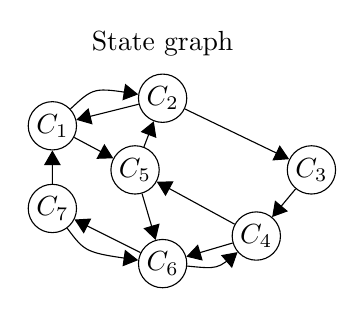
\begin{tikzpicture}[scale=0.7,inner sep=0.4mm
]
\node (c1) [stt] at (4,1.5) {$C_1$};
\node (c2) [stt] at (6,2) {$C_2$};
\node (c3) [stt] at (8.7,0.7) {$C_3$};
\node (c4) [stt] at (7.7,-0.5) {$C_4$};
\node (c5) [stt] at (5.5,0.7) {$C_5$};
\node (c6) [stt] at (6,-1) {$C_6$};
\node (c7) [stt] at (4,0) {$C_7$};
\node (State graph) [] at (6,3) {$$State graph$$};


\draw[-triangle 60] (c2) -- node [] {} (c1);
\draw[-triangle 60] (c2) -- node [] {} (c3);
\draw[-triangle 60] (c3) -- node [] {} (c4);
\draw[-triangle 60] (c4) -- node [] {} (c6);
\draw[-triangle 60] (c6) -- node [] {} (c7);
\draw[-triangle 60] (c7) -- node [] {} (c1);
\draw[-triangle 60] (c1) -- node [] {} (c5);
\draw[-triangle 60] (c4) -- node [] {} (c5);
\draw[-triangle 60] (c5) -- node [] {} (c2);
\draw[-triangle 60] (c5) -- node [] {} (c6);

%krzywe
\draw[-triangle 60] (c6) .. node [] {} controls (7,-1.1) and (7,-1.1)  .. (c4);
\draw[-triangle 60] (c7) .. node [] {} controls (4.6,-0.8) and (4.6,-0.8)  .. (c6);
\draw[-triangle 60] (c1) .. node [] {} controls (4.75,2.2) and (4.75,2.2)  .. (c2);



 
\end{tikzpicture}



\end{document}